\documentclass[../../compsys.tex]{subfiles}
\begin{document}
\chapter{Input/Output Systems}
In this lecture, we will discuss how computers communicate with I/O devices, the layered structure of I/O operations, and the various mechanisms used to optimize I/O performance. \\
\textit{This was mostly covered in Computer Architecture.}

\section{I/O System Architecture}

\subsection{Layered Approach to I/O Operations}
I/O operations in modern computing systems follow a layered approach, with each layer providing a specific set of responsibilities: \\[5px]
\noindent 
\begin{minipage}{0.45\textwidth}
\begin{itemize}
    \item[-] \textbf{Application Layer:} Programs that need to read or write data
    \item[-] \textbf{Library Layer:} Standard libraries that provide I/O functions to applications
    \item[-] \textbf{Operating System Layer:} File systems and device drivers that translate generic operations into device-specific commands
    \item[-] \textbf{Hardware Layer:} Physical devices that perform the actual I/O operations
\end{itemize}
\end{minipage}
\hfill
\vline
\hfill
\begin{minipage}{0.45\textwidth}
\begin{center}
  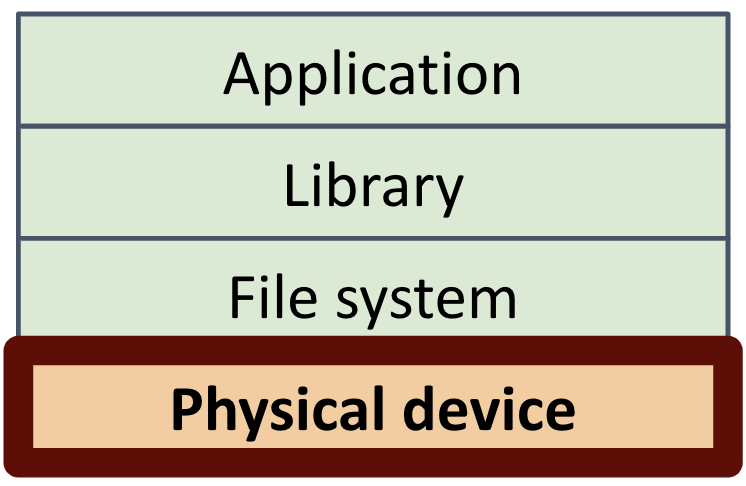
\includegraphics[width=0.6\textwidth]{chapters/L8/images/layers.png}
\end{center}
\end{minipage}\\[7px]
This layered architecture provides abstraction, allowing applications to perform I/O operations without understanding the underlying hardware details.

\subsection{Core I/O Services in Operating Systems}
Operating systems provide several essential I/O services:
\begin{itemize}
    \item[-] Loading programs and data from storage devices
    \item[-] Writing data to display devices (terminals, screens)
    \item[-] Reading and writing network packets
    \item[-] Capturing input from various input devices (keyboard, mouse, sensors)
\end{itemize}

These services form the foundation of how users and applications interact with the computer system.

\section{Device Interaction Models}

\subsection{Canonical Device Structure}
Device communication follows a standardized model that abstracts hardware complexity:\\[5px]

\begin{definition}[Canonical Device]
A \textbf{canonical device} refers to a standardized model of I/O device interaction where the CPU communicates with a device controller through designated registers, while the internal workings of the device remain hidden from the system.
\end{definition}
\vspace{5px}
\begin{center}
  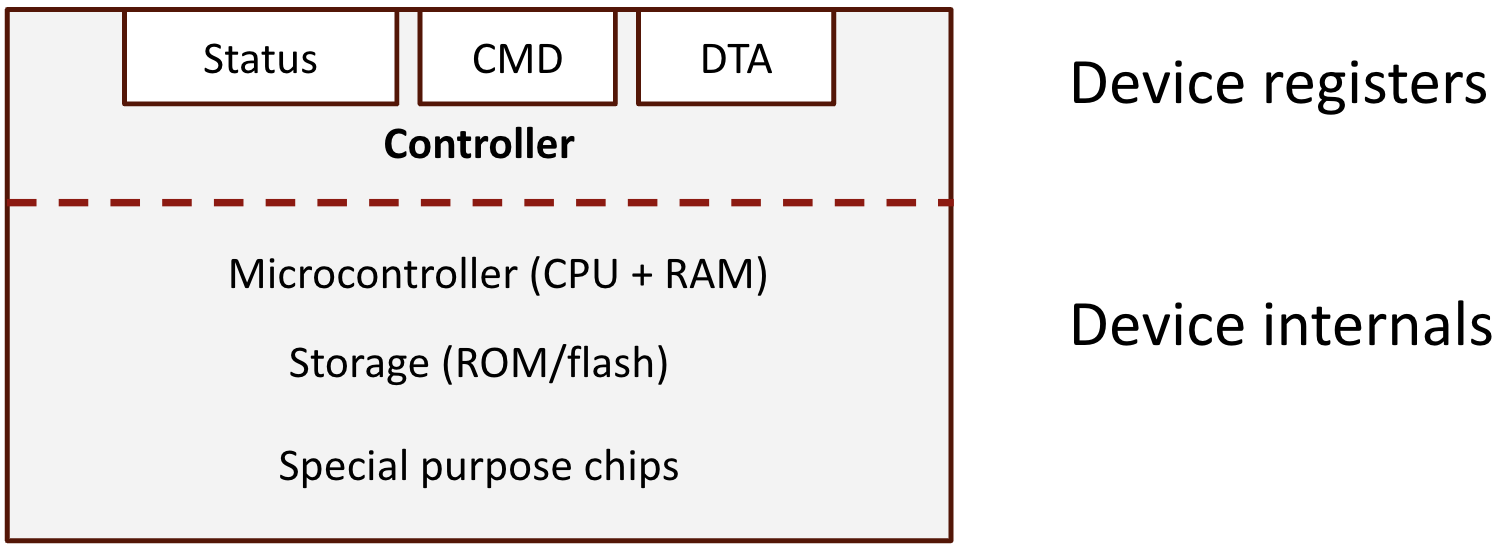
\includegraphics[width=0.45\textwidth]{chapters/L8/images/canonical_device.png}
\end{center}

In this interaction, we have the following components:
\begin{itemize}
    \item[-] \textbf{Device Controller:} Hardware that interfaces between the device and the system
    \item[-] \textbf{Device Registers:} Control, status, and data registers used for communication
    \item[-] \textbf{Device Driver:} Software component that knows how to communicate with specific devices
    \item[-] \textbf{Signaling Mechanisms:} Methods (polling or interrupts) for the device to signal its status to the CPU
\end{itemize}


\begin{justify}
\textbf{Question:} Why do we setup data before setting up the CMD register? \\[5px]
\textbf{Answer:} Race condition if data is not present
\end{justify}

\begin{definition}[Race Condition]
    \leavevmode \\
    A \textbf{race condition} occurs when the timing or ordering of events affects the correctness of a program. In device interactions, setting up data before the command prevents race conditions where the device might begin execution before all necessary data is available.
\end{definition}
\vspace{10px}

Thus the following steps are taken to communicate with the device:\\[5px]
\begin{minipage}{0.45\textwidth}
    \begin{enumerate}
        \item Wait until the device is ready (check status register)
        \item Set data in the data register
        \item Issue command by writing to the command register
        \item Wait for command completion (check status register)
    \end{enumerate}
\end{minipage}
\hfill
\vline
\hfill
\begin{minipage}{0.45\textwidth}
    \begin{cc}
// 1. Wait until device is ready
while (STATUS == BUSY) ;

// 2. Write data to data register
*dtaRegister = DATA;

// 3. Write command to command register
*cmdRegister = COMMAND;

// 4. Wait until command completes
while (STATUS == BUSY) ;
\end{cc}
\end{minipage}

\newpage
\section{Parameters of I/O Operations}

When designing or analyzing I/O systems, five fundamental parameters must be considered:

\begin{enumerate}
    \item \textbf{Communication Method:} How does the CPU communicate with the device?
    \item \textbf{Data Granularity:} What is the size of data transfers (byte, block, etc.)?
    \item \textbf{Access Pattern:} How is data accessed (sequentially or randomly)?
    \item \textbf{Notification Mechanism:} How does the device signal the CPU?
    \item \textbf{Transfer Mechanism:} How is data moved between memory and device?
\end{enumerate}

\subsection{CPU-Device Communication: Memory-Mapped I/O}

\begin{definition}[Memory-Mapped I/O (MMIO)]
\textbf{Memory-Mapped I/O (MMIO)} is a method where device control registers are mapped into the physical address space of the processor, allowing the CPU to access devices using standard memory access instructions (load/store).
\end{definition}
\vspace{10px}
\begin{minipage}[htp]{0.45\textwidth}
    In Memory-Mapped I/O, we have the following characteristics:
    \begin{itemize}
        \item Device registers appear as memory locations to the CPU
        \item Standard load/store instructions are used for device communication
        \item Applicable to a wide range of devices
        \item Particularly effective for high-performance devices (fast storage, network interfaces, displays)
    \end{itemize}
\end{minipage}
\hfill
\vline
\hfill
\begin{minipage}[htp]{0.45\textwidth}
    \begin{center}
        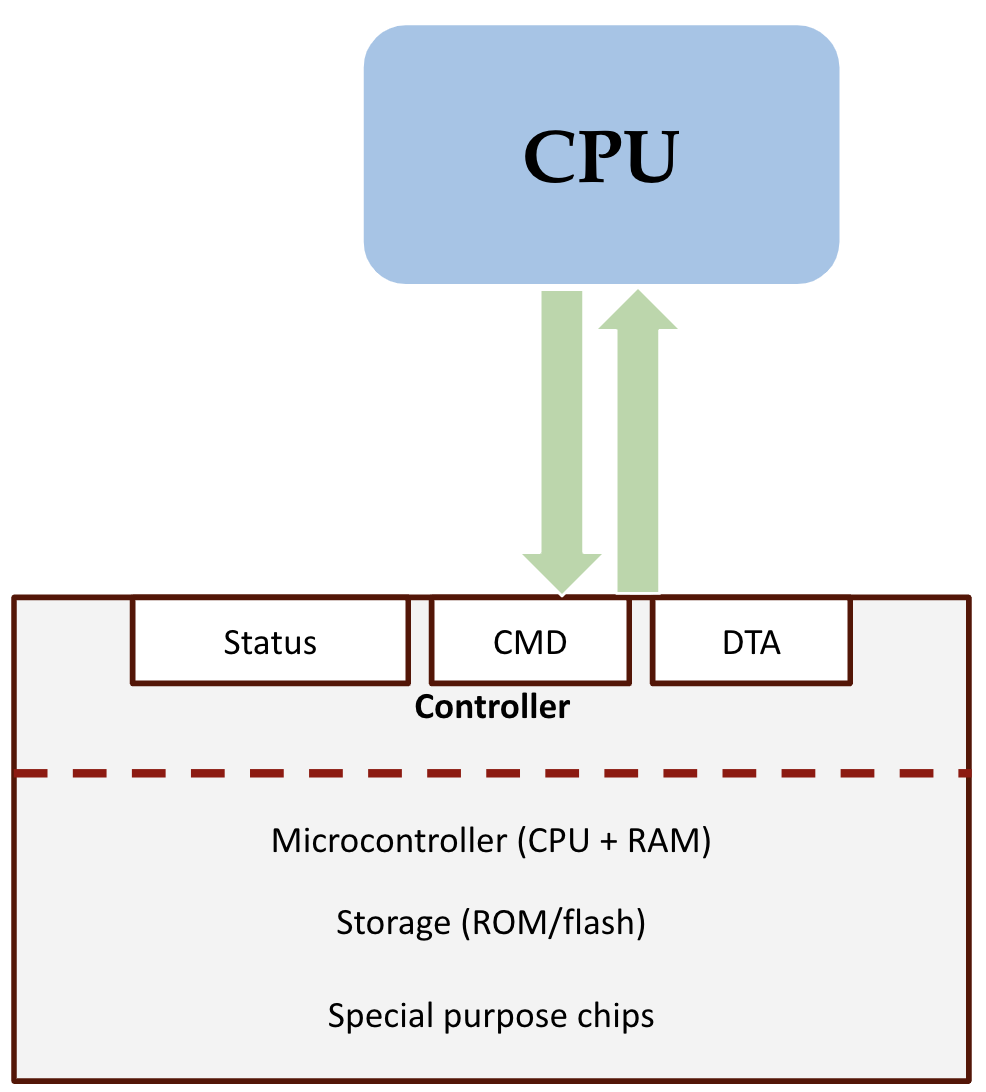
\includegraphics[width=0.75\textwidth]{chapters/L8/images/mmio.png}
    \end{center}
\end{minipage}


\subsection{Data Granularity and Access Patterns}

Different I/O devices operate with different data sizes and access patterns:

\begin{itemize}
    \item \textbf{Data Granularity:}
    \begin{itemize}
        \item \textit{Byte-oriented devices:} Transfer one byte at a time (e.g., keyboards, serial ports)
        \item \textit{Block-oriented devices:} Transfer blocks of data (e.g., disk drives, network cards)
    \end{itemize}

    \item \textbf{Access Patterns:}
    \begin{itemize}
        \item \textit{Sequential access:} Data must be accessed in order (e.g., tape drives)
        \item \textit{Random access:} Data can be accessed in any order (e.g., disk drives, SSDs)
    \end{itemize}
\end{itemize}

These characteristics significantly impact the design of device drivers and the overhead involved in data transfers.

\section{Notification Mechanisms}

\subsection{From Polling to Interrupts}

Waiting for device operations to complete poses a challenge for system efficiency. Two main approaches address this:

\begin{center}
  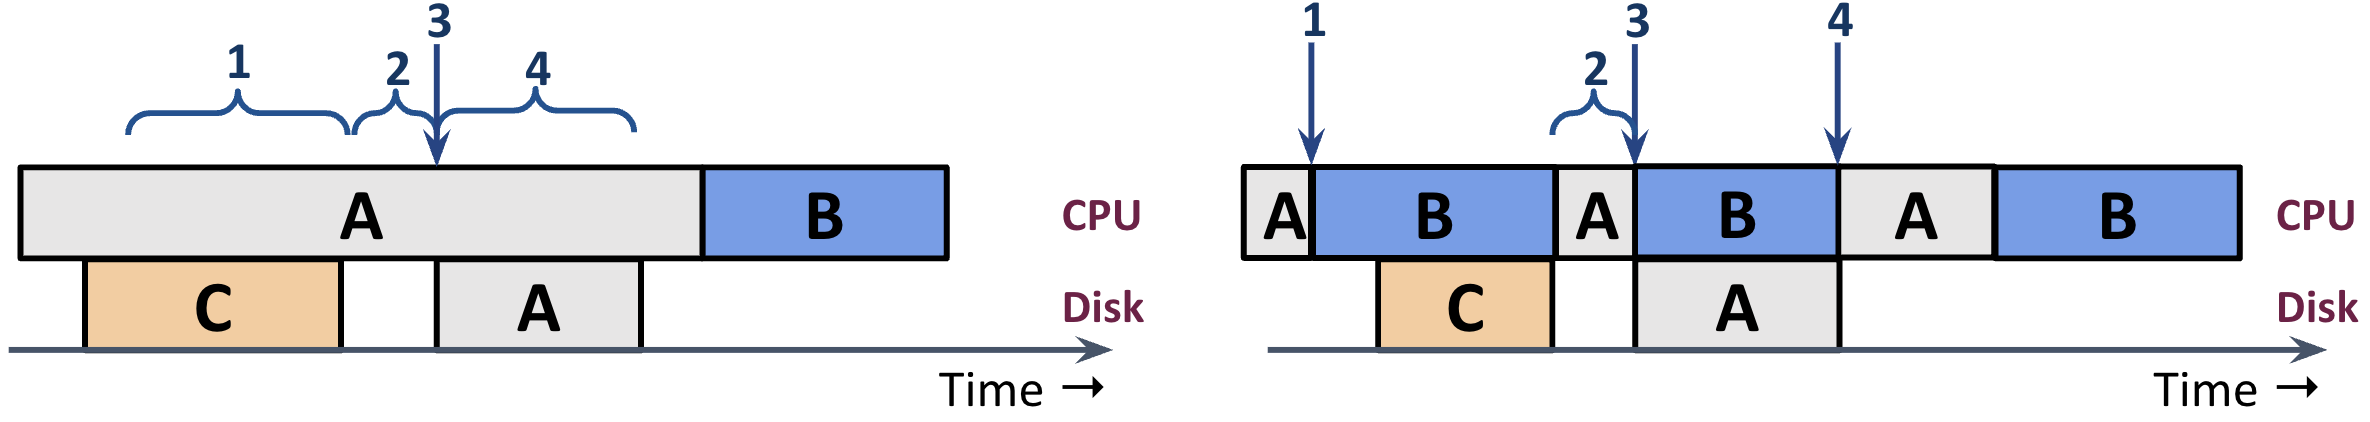
\includegraphics[width=0.75\textwidth]{chapters/L8/images/device_protocol.png}
\end{center}

\begin{definition}[Polling]
\textbf{Polling} (or busy-waiting) is a notification technique where the CPU periodically checks a device's status register to determine if an operation has completed.
\end{definition}
\vspace{10px}
\begin{definition}[Interrupt]
An \textbf{interrupt} is a hardware signal sent from a device to the CPU that causes the CPU to temporarily suspend its current execution, save its state, and execute an interrupt handler routine.
\end{definition}

\subsection{Comparing Polling and Interrupts}

\begin{table}[h]
\centering
\begin{tabular}{|p{2.5cm}|p{5cm}|p{5cm}|}
\hline
\textbf{Aspect} & \textbf{Polling} & \textbf{Interrupts} \\
\hline
Mechanism & CPU periodically checks device status & Device signals CPU when attention needed \\
\hline
CPU Utilization & Wastes CPU cycles when events are infrequent & Efficient for unpredictable or infrequent events \\
\hline
Overhead & Low per-check overhead & Higher overhead for context switching \\
\hline
Predictability & Predictable timing & Less predictable \\
\hline
Best Use Cases & High-frequency events, short wait times & Unpredictable events, long wait times \\
\hline
\end{tabular}
\end{table}

\begin{definition}[Livelock]
\textbf{Livelock} is a situation where a system is continuously responding to interrupts and cannot make progress on its main tasks, similar to deadlock but with processes actively running rather than blocked.
\end{definition}

\subsection{Optimizing Notification Mechanisms}

Modern systems use sophisticated approaches to balance efficiency:

\begin{itemize}
    \item[-] \textbf{Hybrid Approaches:} Using both polling and interrupts depending on workload characteristics
    \item[-] \textbf{Interrupt Coalescing:} Delaying and batching multiple interrupts to reduce overhead
    \item[-] \textbf{Adaptive Strategies:} Dynamically switching between polling and interrupts based on system load and device activity
\end{itemize}

\subsection{Data Transfer Mechanisms}

The final aspect of I/O operations concerns how data is transferred between main memory and device controllers.

\begin{definition}[Programmed I/O (PIO)]
\textbf{Programmed I/O (PIO)} is a data transfer technique where the CPU directly controls data movement between memory and a device, executing an instruction for each data unit transferred.
\end{definition}

\begin{definition}[Direct Memory Access (DMA)]
\textbf{Direct Memory Access (DMA)} is a data transfer technique that allows a device controller to directly transfer data to or from main memory without CPU intervention, after initial setup by the CPU.
\end{definition}

\begin{center}
\begin{tabular}{|p{2.5cm}|p{5cm}|p{5cm}|}
\hline
\textbf{Aspect} & \textbf{Programmed I/O} & \textbf{Direct Memory Access} \\
\hline
CPU Involvement & CPU handles each data transfer & CPU only sets up transfer, then free for other tasks \\
\hline
Efficiency & Efficient for small transfers & Efficient for large transfers \\
\hline
Complexity & Simpler implementation & More complex hardware needed \\
\hline
CPU Overhead & High, proportional to data size & Low, independent of data size \\
\hline
Best Use Cases & Small data transfers, simple devices & Large data transfers, high-performance devices \\
\hline
\end{tabular}
\end{center}
\begin{itemize}
    \item[-] \textbf{Programmed I/O (PIO):}
    \begin{itemize}
        \item CPU directly controls data transfer, telling the device what data is
        \item Requires one instruction for each byte/word transferred
        \item Efficient for small transfers but consumes CPU cycles proportional to data size
    \end{itemize}
    \item[-] \textbf{Direct Memory Access (DMA):}
    \begin{itemize}
        \item CPU only tells the device where data is located in memory
        \item Controller is granted access to the memory bus
        \item Device transfers data to/from memory without CPU intervention
        \item Highly efficient for large data transfers
    \end{itemize}
\end{itemize}

\section{Direct Memory Access (DMA)}

\begin{definition}[Direct Memory Access (DMA)]
Direct Memory Access (DMA) is a method that allows hardware subsystems to access main system memory independently of the CPU, enabling efficient data transfer between I/O devices and memory.
\end{definition}

\subsection{DMA Controller Operation}

The DMA controller facilitates direct data transfer between peripheral devices and memory without constant CPU intervention, significantly improving system efficiency for data-intensive operations.

\begin{minipage}{0.45\textwidth}
The following steps illustrate a typical DMA transfer sequence:
\begin{enumerate}
    \item The device driver receives an instruction to transfer disk data to a buffer at address X.
    \item The driver commands the disk controller to transfer C bytes from disk to the buffer at address X.
    \item The disk controller initiates the DMA transfer operation.
    \item The disk controller sends each byte to the DMA controller.
    \item The DMA controller transfers bytes to buffer X, incrementing the memory address and decrementing C until C = 0.
    \item When C = 0, the DMA controller interrupts the CPU to signal completion of the transfer.
\end{enumerate}
\end{minipage}
\hfill
\vline
\hfill
\begin{minipage}{0.45\textwidth}
\begin{center}
    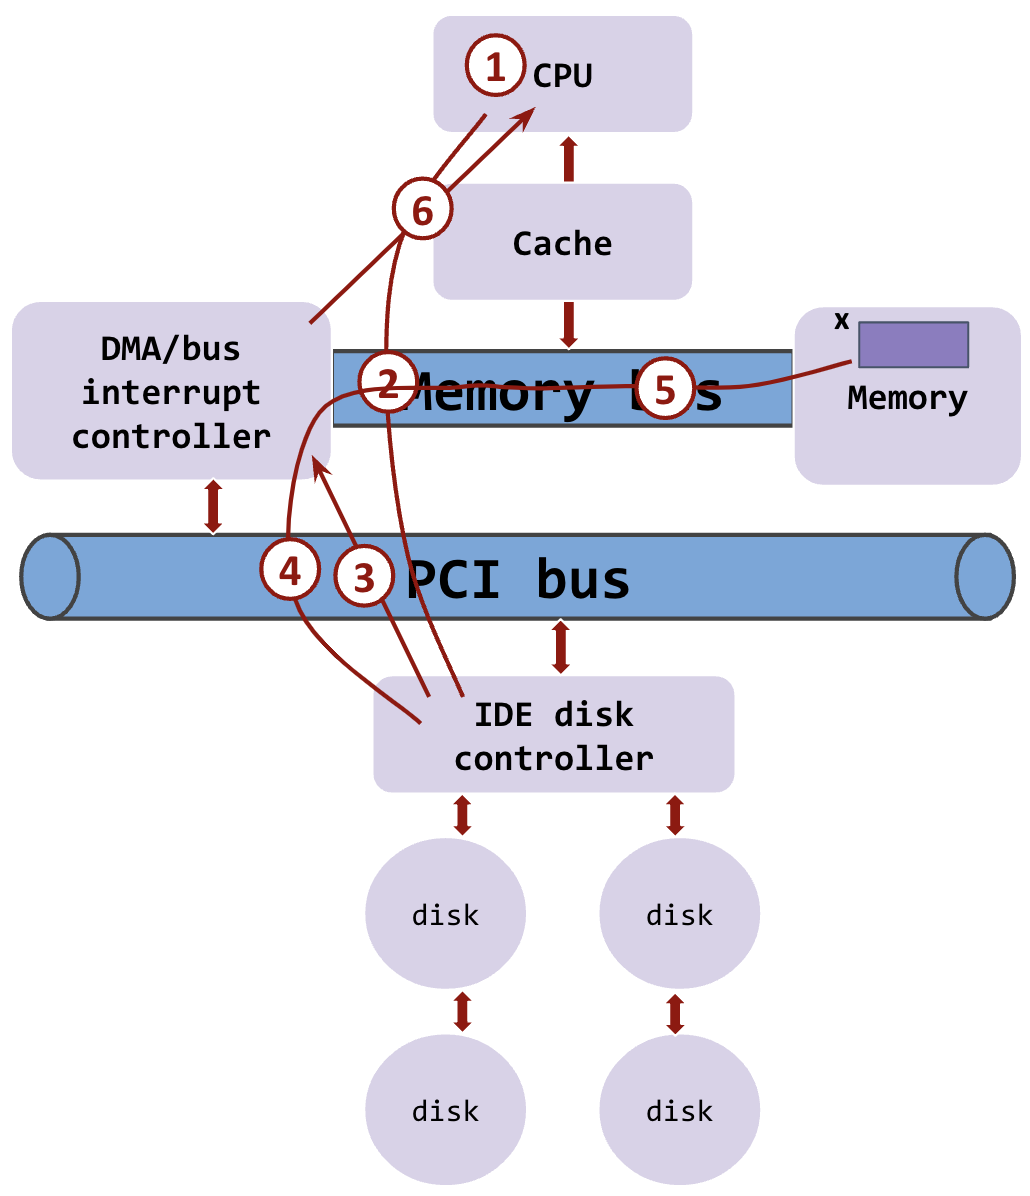
\includegraphics[width=0.85\textwidth]{chapters/L8/images/dma.png}
\end{center}
\end{minipage}

\section{Device Management in Operating Systems}

\subsection{The Device Driver Challenge}

Modern computing systems must interface with numerous devices, each with unique protocols and requirements. This diversity creates significant challenges for operating system design.

\begin{definition}[Device Driver]
A device driver is a specialized component of the operating system kernel that directly interfaces with hardware devices, translating between the standardized OS interfaces and device-specific protocols.
\end{definition}

Device drivers solve the challenge of hardware diversity by:
\begin{itemize}
    \item Supporting a standard, internal interface within the OS
    \item Enabling the same kernel I/O system calls to interact with different physical devices
    \item Providing device-specific implementations of standard operations
\end{itemize}

\subsection{Principles of Device Driver Design}

Device drivers demonstrate encapsulation in system design. Different drivers adhere to the same API, allowing the OS to interact with diverse hardware through consistent interfaces. The OS implements support for APIs based on device class rather than specific hardware models.

This approach requires:
\begin{itemize}
    \item Well-designed interfaces and APIs
    \item Careful balance between versatility and specialization
    \item Layered API structure to manage complexity
\end{itemize}

\subsection{Complexity of API Layers}

The file system stack exemplifies the layered approach to I/O management:

\begin{center}
    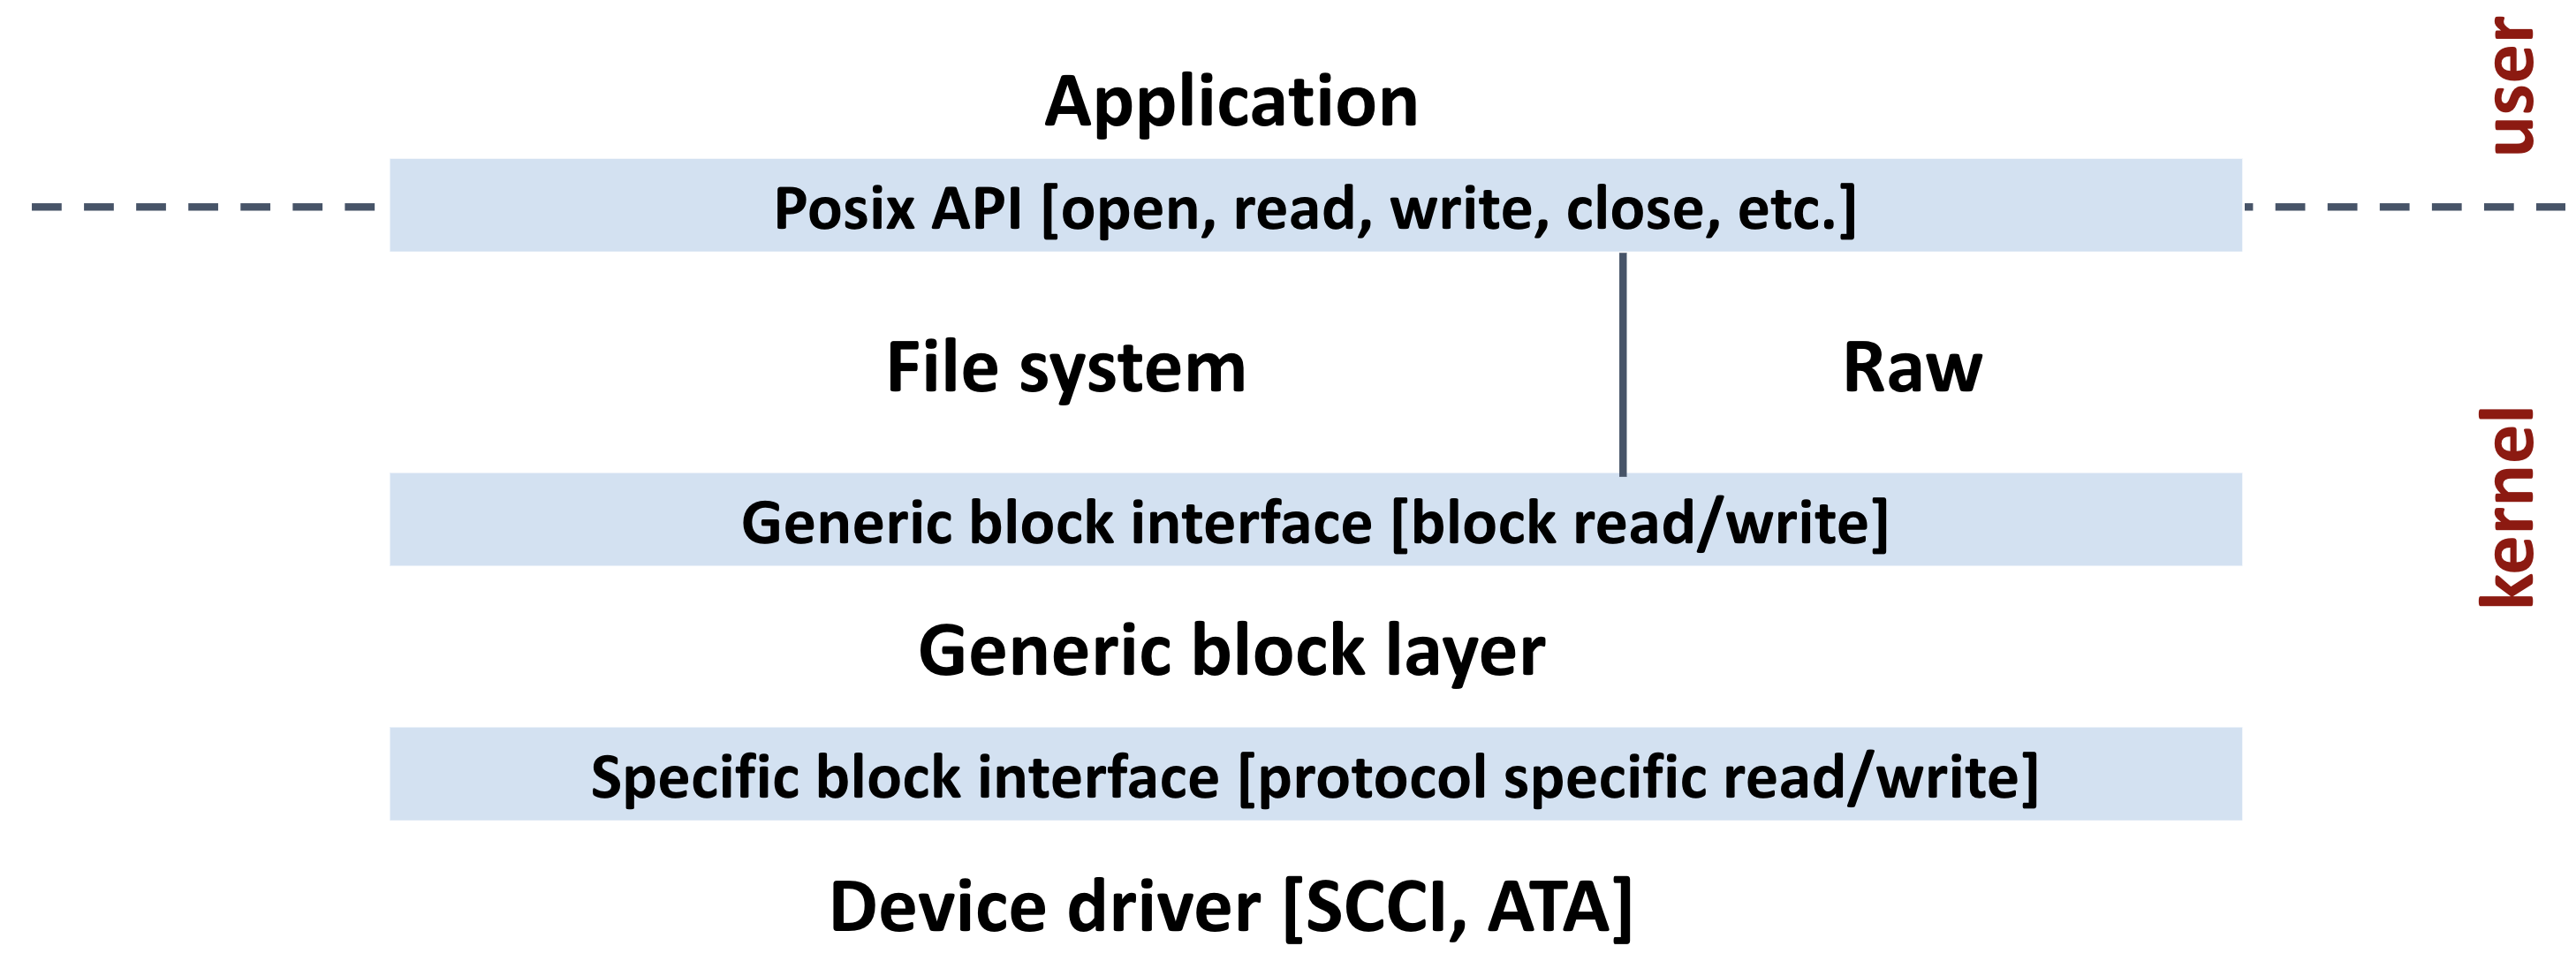
\includegraphics[width=0.65\textwidth]{chapters/L8/images/fs-api.png}
\end{center}

This layering allows for abstraction and modularity while providing necessary functionality at each level.

\subsection{OS Device Structure}

The overall device structure in an operating system organizes components into logical layers:

\begin{center}
    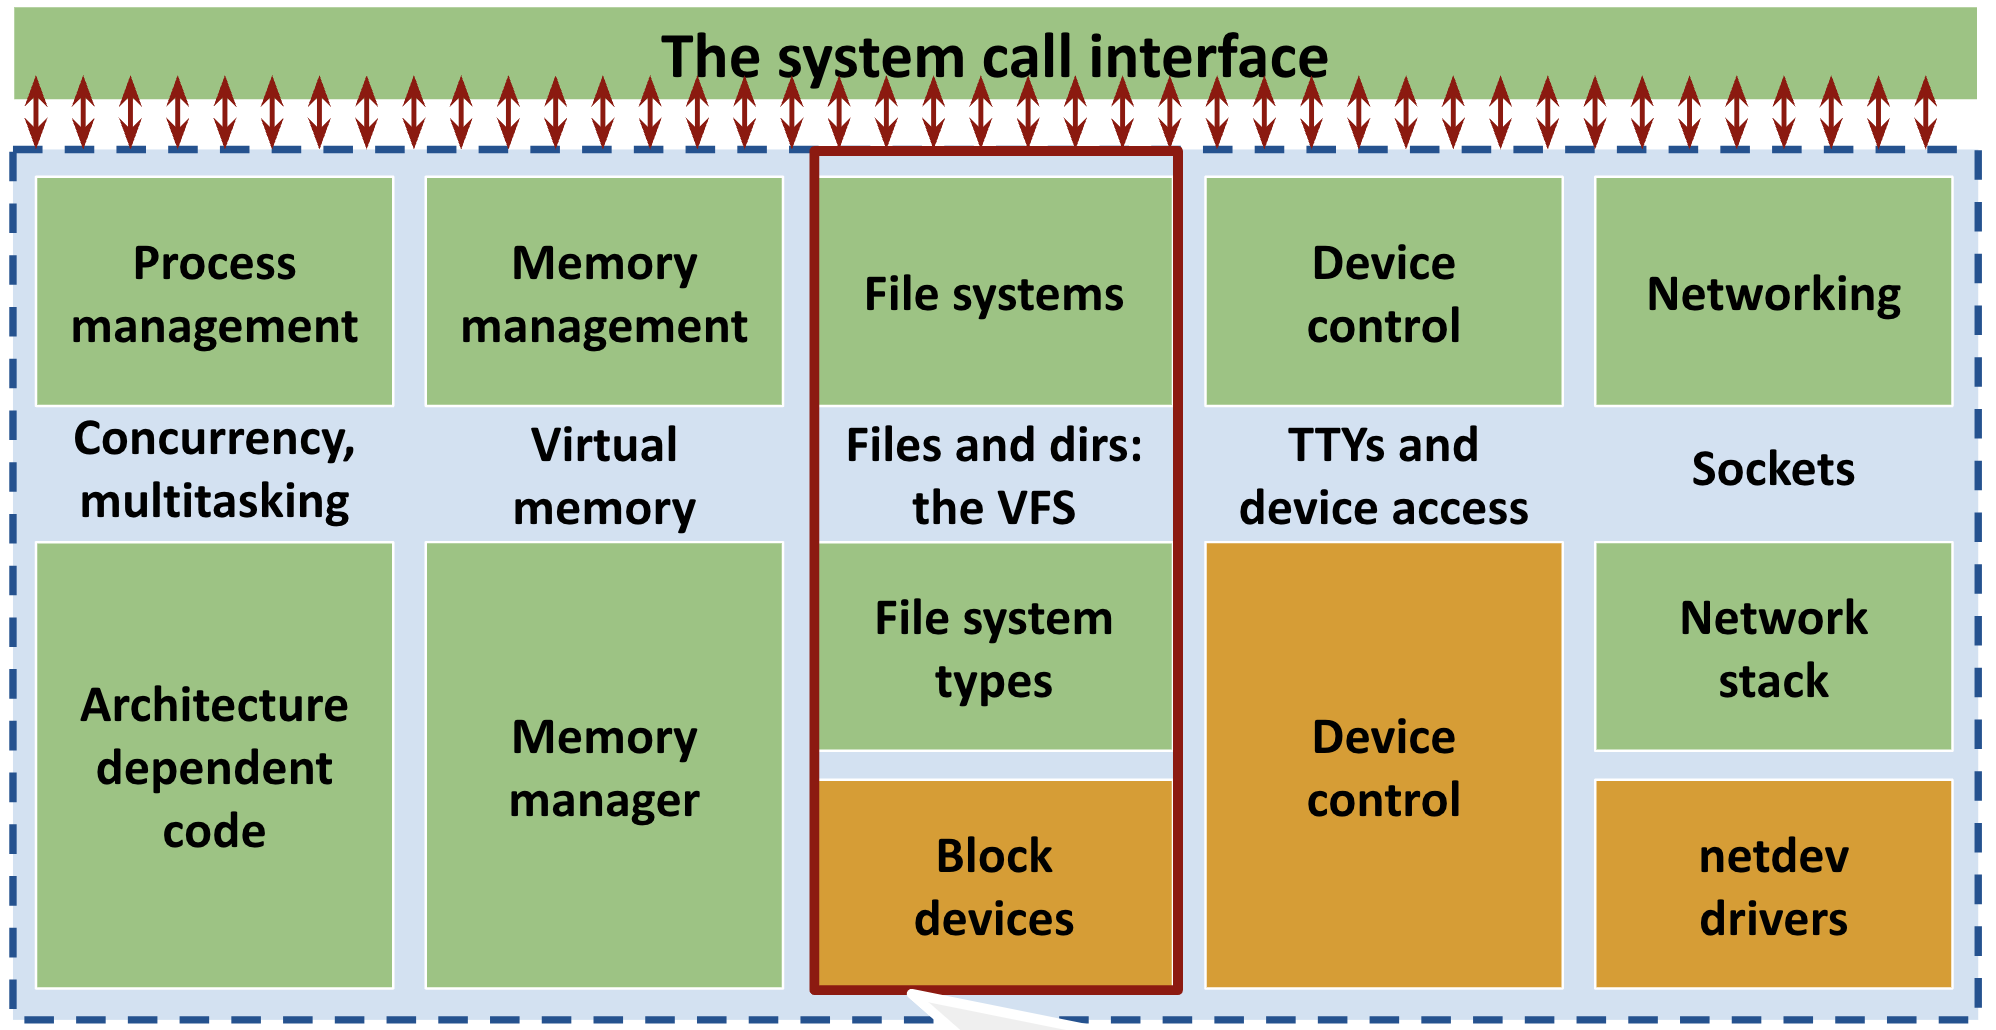
\includegraphics[width=0.65\textwidth]{chapters/L8/images/os.png}
\end{center}


\begin{itemize}
    \item \textbf{Process Management:} Handles process creation, scheduling, synchronization, and termination, allowing multiple programs to run concurrently.
    
    \item \textbf{Memory Management:} Controls allocation and deallocation of memory resources, implements virtual memory, and manages address translation.
    
    \item \textbf{File Systems:} Provides abstractions for persistent data storage, organizing files and directories while managing access permissions.
    
    \item \textbf{Device Control:} Interfaces with hardware peripherals through device drivers, translating generic commands into device-specific operations.
    
    \item \textbf{Networking:} Implements network protocols and provides interfaces for network communication, enabling data exchange between systems.
\end{itemize}

The system call interface serves as the boundary between user applications and these kernel components, providing a standardized way for programs to request services from the operating system. Through system calls, applications can interact with all these subsystems without needing to understand their internal implementation details.

\subsection{General I/O Abstraction Stack}
I/O systems are accessed through a series of layered abstractions that progressively translate between user-level operations and hardware-specific details:

\begin{minipage}{0.45\textwidth}
        These layers provide:
        \begin{itemize}
            \item Caching of recently read disk blocks
            \item Buffering of recently read blocks
            \item A unified interface to diverse devices
            \item Fixed-size block data operations
            \item Translation between OS abstractions and hardware-specific details
            \item Control of hardware registers, bulk data transfers, and OS notifications
        \end{itemize}

\end{minipage}
\hfill
\vline
\hfill
\begin{minipage}{0.45\textwidth}
    \begin{center}
        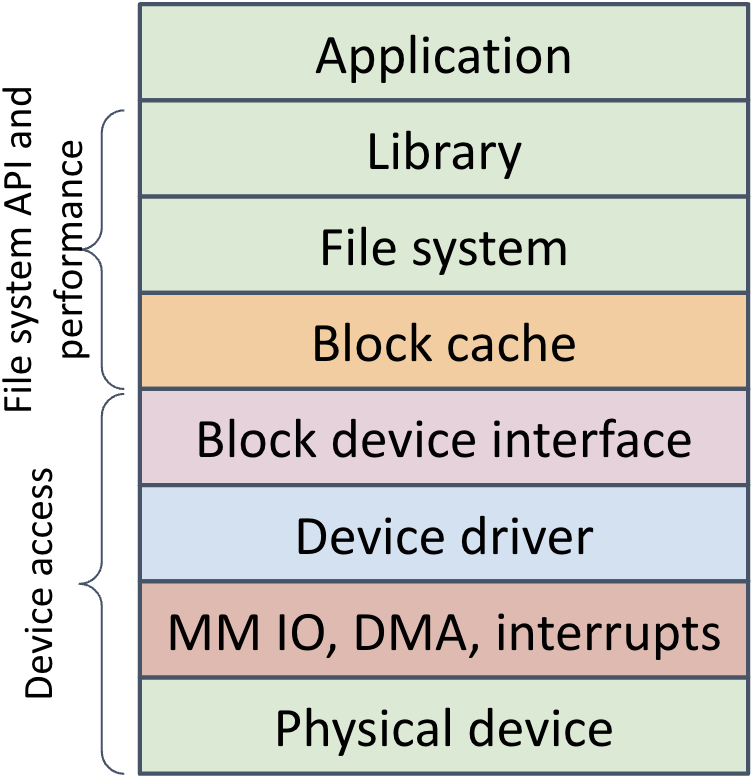
\includegraphics[width=0.75\textwidth]{chapters/L8/images/io-stack.png}
    \end{center}
\end{minipage}

\section{Storage Systems}

\subsection{Storage Media Evolution}

\begin{definition}[Persistent Storage]
Persistent storage refers to data storage technologies that retain information even when power is removed from the system.
\end{definition}
\vspace{5px}
Computer systems have employed various storage media for persistent data:\\[8px]
\begin{minipage}{0.45\textwidth}
\begin{itemize}
    \item[-] Punched paper cards
    \item[-] Magnetic tapes
    \item[-] Floppy disks
    \item[-] Magnetic hard disks
\end{itemize}
\end{minipage}
\hfill
\begin{minipage}{0.45\textwidth}
\begin{itemize}
    \item[-] Optical disks
    \item[-] USB flash drives
    \item[-] Solid-state drives
\end{itemize}
\end{minipage}

\subsection{The Storage Hierarchy}

Modern computing systems organize storage into a hierarchy based on speed, capacity, and cost: \\
\textit{Main memory for currently used data} and \textit{Disk for storing application data}
\begin{center}
    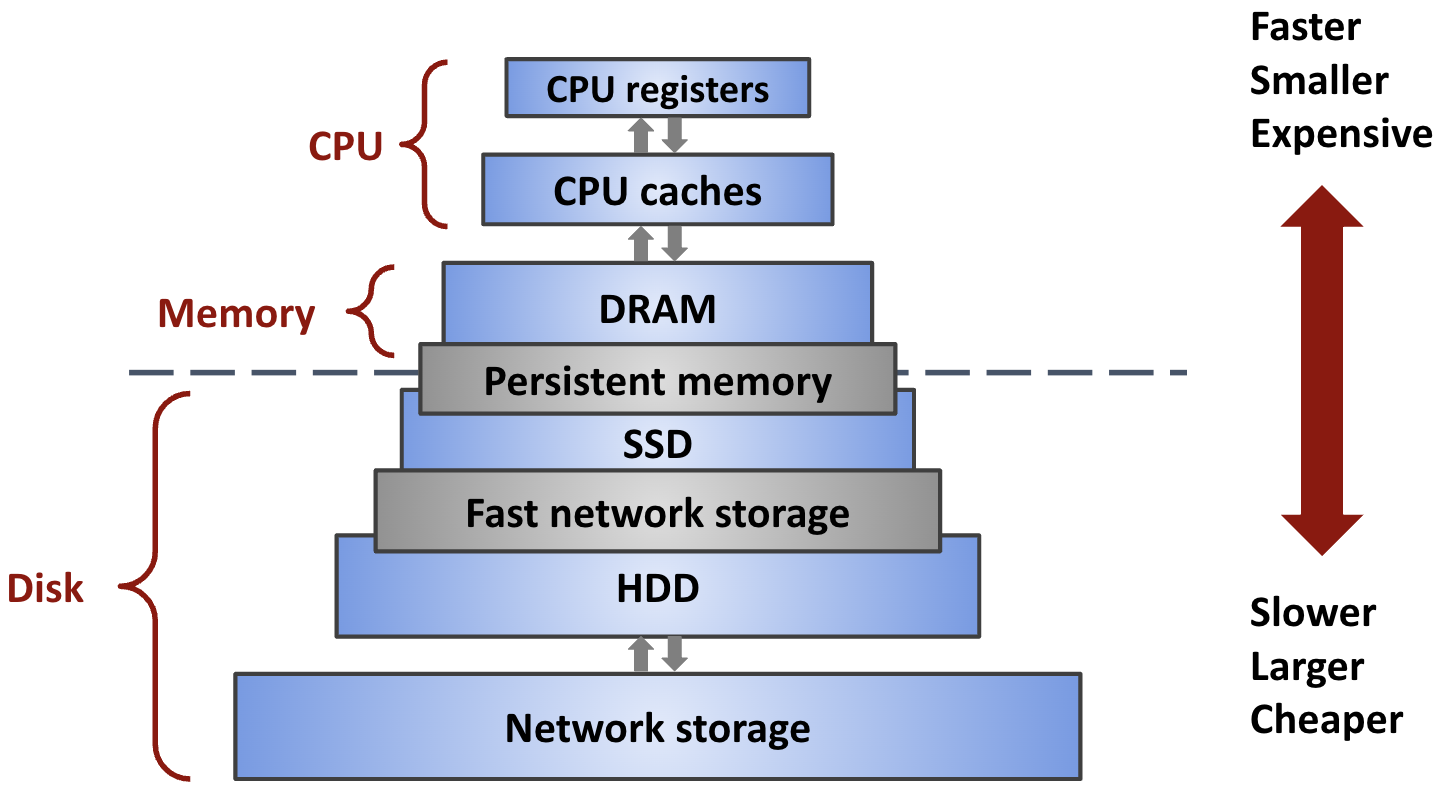
\includegraphics[width=0.55\textwidth]{chapters/L8/images/hierarchy.png}
\end{center}

\newpage
\subsection{Performance Considerations: Latency}

Understanding storage performance requires awareness of access latency across different technologies:

\begin{center}
    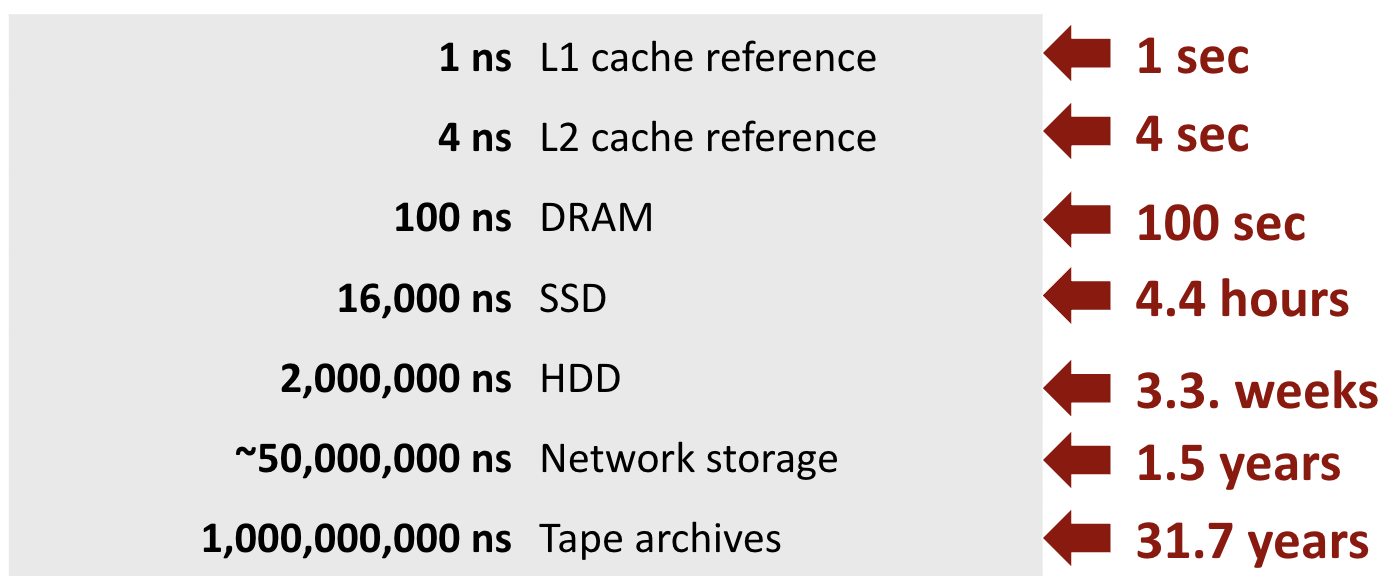
\includegraphics[width=0.55\textwidth]{chapters/L8/images/latency.png}
\end{center}

These latency figures are critical knowledge for system designers and software engineers when optimizing data access patterns.

\subsection{Disk Storage Characteristics}

Magnetic and solid-state disks serve as the predominant secondary storage devices in modern systems:

\begin{definition}[Disk Block]
A disk block (or page) is the fundamental unit of data storage and retrieval for disk-based storage systems.
\end{definition}

Key characteristics of disk storage include:
\begin{itemize}
    \item Non-uniform access times, unlike RAM
    \item Access time variations based on disk technology (magnetic vs. flash)
    \item Performance differences between sequential and random access patterns
\end{itemize}

The relative placement of data on physical disks significantly impacts application performance, making storage optimization a critical consideration in system design.

\subsection{Data Integrity in Storage Systems}

Modern storage systems employ various techniques to ensure data integrity:
\begin{itemize}
    \item Error detection and correction codes to handle bit errors
    \item Capabilities to detect data corruption
    \item Error handling at both controller and OS levels
\end{itemize}

Despite these safeguards, storage devices remain a potential single point of failure in computing systems, with limitations in performance, capacity, and reliability.
\newpage
\section{Redundant Array of Inexpensive Disks (RAID)}

\begin{definition}[Redundant Array of Inexpensive Disks (RAID)]
RAID (Redundant Array of Inexpensive Disks) is a storage virtualization technology that combines multiple physical disk drives into a single logical unit for improved performance, capacity, or reliability.
\end{definition}

\subsection{Storage System Requirements}

Effective storage systems must satisfy three key requirements:
\begin{itemize}
    \item[-] Speed: Data must be accessible with minimal latency
    \item[-] Reliability: Retrieved data must match what was originally stored
    \item[-] Affordability: Cost must be reasonable relative to system requirements
\end{itemize}

RAID technology addresses these requirements by building logical storage volumes from multiple physical disks, providing:
\begin{itemize}
    \item[-] Higher throughput through data striping
    \item[-] Improved reliability through redundancy
    \item[-] Cost-effective scaling of storage capacity
\end{itemize}

\subsection{RAID 0: Striping}
RAID 0 focuses on performance optimization by distributing data across multiple disks, allowing parallel access to improve throughput and reduce access times.

\begin{definition}[RAID 0]
RAID 0 implements block-level striping without parity or mirroring, distributing data evenly across multiple disks without redundancy.
\end{definition}

\begin{minipage}{0.45\textwidth}

    Characteristics of RAID 0:
    \begin{itemize}
        \item Files are striped across multiple disks
        \item No data redundancy or fault tolerance
        \item Provides maximum performance and full storage capacity
        \item Cumulative bandwidth across all member disks
        \item Total storage capacity equals the sum of all disk capacities
        \item Reduced reliability as disk count increases (higher probability of failure)
    \end{itemize}
\end{minipage}
\hfill
\vline
\hfill
\begin{minipage}{0.45\textwidth}
    \begin{center}
        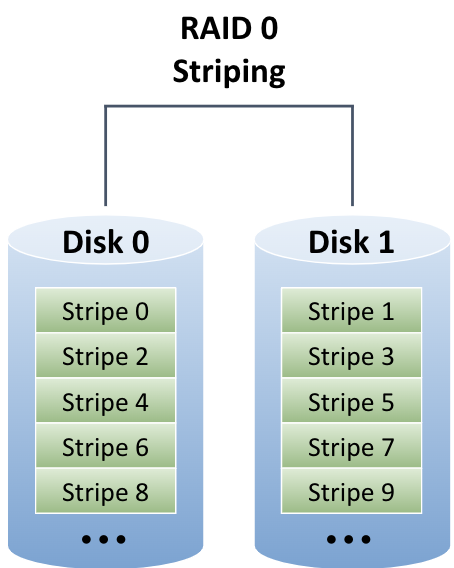
\includegraphics[width=0.65\textwidth]{chapters/L8/images/raid0.png}
    \end{center}
\end{minipage}
\begin{example}
In a four-disk RAID 0 array, each with a mean time between failures (MTBF) of 100,000 hours, the expected MTBF for the entire array would be approximately 25,000 hours (one-fourth of a single disk's MTBF), since failure of any single disk results in data loss for the entire array.
\end{example}

\subsection{RAID 1: Mirroring}
RAID 1 focuses on data reliability through complete redundancy, creating exact copies of data across multiple disks to protect against hardware failures. \\[5px]
\begin{definition}[RAID 1]
    RAID 1 implements disk mirroring, where identical data is written to two or more drives, providing complete data redundancy.
\end{definition}
\vspace{5px}
\begin{minipage}{0.45\textwidth}
    \small
    Characteristics of RAID 1:
    \begin{itemize}
        \item Data blocks are duplicated across multiple drives
        \item Excellent protection against disk failure
        \item Does not protect against data corruption
        \item Usable storage capacity equals that of a single disk
        \item Read operations can be parallelized
        \item Write performance equivalent to a single disk
        \item Higher cost per usable gigabyte
        \item Commonly used for critical systems and sensitive information
    \end{itemize}   
\end{minipage}
\hfill
\vline
\hfill
\begin{minipage}{0.45\textwidth}
    \begin{center}
        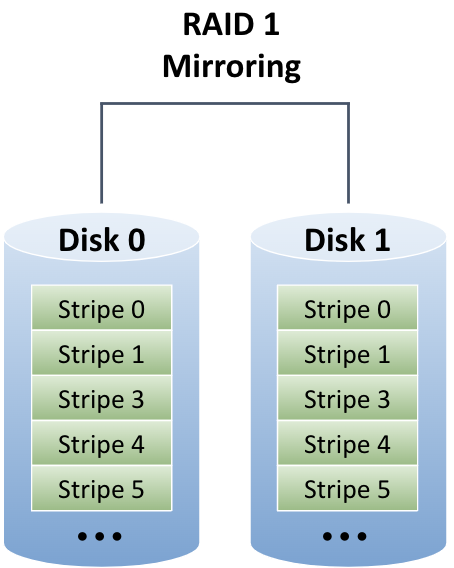
\includegraphics[width=0.65\textwidth]{chapters/L8/images/raid1.png}
    \end{center}
\end{minipage}

\subsection{RAID 5: Distributed Parity}
RAID 5 balances performance and reliability by distributing both data and parity information across all disks in the array, providing fault tolerance with better storage efficiency than mirroring.\\[5px]
\begin{minipage}{0.45\textwidth}
    \small
    RAID 5 has the following features:
    \begin{itemize}
        \item[-] Distributed parity blocks across all disks
        \item[-] Can survive failure of any single disk
        \item[-] Data can be reconstructed using XOR operations on remaining drives
        \item[-] Good read performance: approximately (N-1) times that of a single disk
        \item[-] Write operations are more complex due to parity calculations
        \item[-] Storage efficiency: usable capacity is (N-1) disks in an N-disk array
        \item[-] Commonly used in data center environments
    \end{itemize}
\end{minipage}
\hfill
\vline
\hfill
\begin{minipage}{0.45\textwidth}
    \begin{center}
        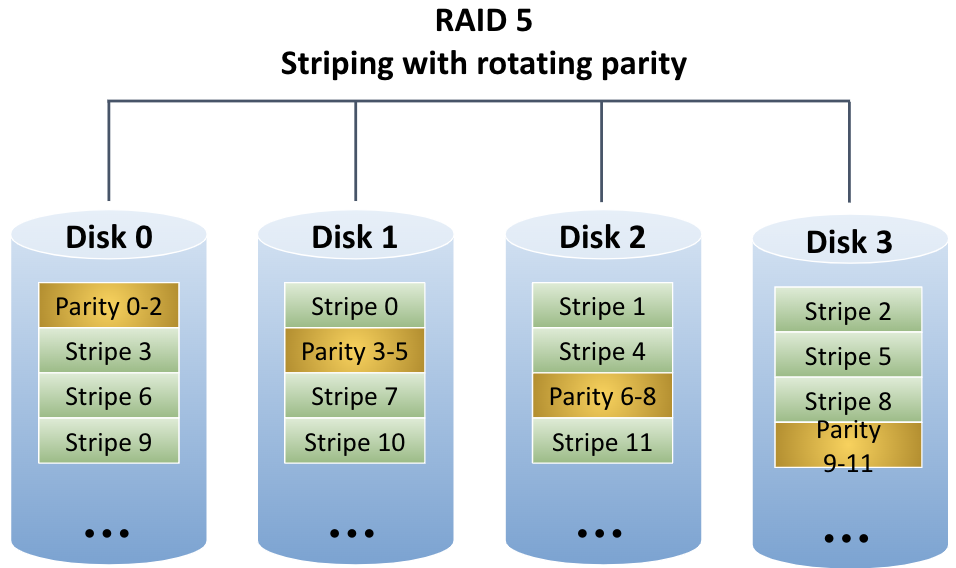
\includegraphics[width=0.95\textwidth]{chapters/L8/images/raid5.png}
    \end{center}
\end{minipage}
\vspace{10px}
\begin{definition}[RAID 5]
RAID 5 implements block-level striping with distributed parity, providing fault tolerance while using less storage for redundancy than mirroring.
\end{definition}

\begin{definition}[Parity]
Parity is a fault tolerance mechanism where redundant data is calculated and stored to enable recovery from single-disk failures. For a set of blocks S$_i$ through S$_j$, the parity P$_{i-j}$ is calculated as: 
$P\_{i-j} = S\_{i} \xor S\_{i+1} \xor ... \xor S\_{j}$, where $\xor$ represents the XOR operation.
\end{definition}


\begin{example}
In a 5-disk RAID 5 array, if disk 3 fails, its data can be reconstructed by performing XOR operations on the corresponding blocks from the other 4 disks. This allows the system to continue operation despite the failure, though with degraded performance until the failed disk is replaced and rebuilt.
\end{example}

\end{document}